\documentclass[11pt]{article}\usepackage[]{graphicx}\usepackage[]{color}
%% maxwidth is the original width if it is less than linewidth
%% otherwise use linewidth (to make sure the graphics do not exceed the margin)
\makeatletter
\def\maxwidth{ %
  \ifdim\Gin@nat@width>\linewidth
    \linewidth
  \else
    \Gin@nat@width
  \fi
}
\makeatother

\definecolor{fgcolor}{rgb}{0.345, 0.345, 0.345}
\newcommand{\hlnum}[1]{\textcolor[rgb]{0.686,0.059,0.569}{#1}}%
\newcommand{\hlstr}[1]{\textcolor[rgb]{0.192,0.494,0.8}{#1}}%
\newcommand{\hlcom}[1]{\textcolor[rgb]{0.678,0.584,0.686}{\textit{#1}}}%
\newcommand{\hlopt}[1]{\textcolor[rgb]{0,0,0}{#1}}%
\newcommand{\hlstd}[1]{\textcolor[rgb]{0.345,0.345,0.345}{#1}}%
\newcommand{\hlkwa}[1]{\textcolor[rgb]{0.161,0.373,0.58}{\textbf{#1}}}%
\newcommand{\hlkwb}[1]{\textcolor[rgb]{0.69,0.353,0.396}{#1}}%
\newcommand{\hlkwc}[1]{\textcolor[rgb]{0.333,0.667,0.333}{#1}}%
\newcommand{\hlkwd}[1]{\textcolor[rgb]{0.737,0.353,0.396}{\textbf{#1}}}%
\let\hlipl\hlkwb

\usepackage{framed}
\makeatletter
\newenvironment{kframe}{%
 \def\at@end@of@kframe{}%
 \ifinner\ifhmode%
  \def\at@end@of@kframe{\end{minipage}}%
  \begin{minipage}{\columnwidth}%
 \fi\fi%
 \def\FrameCommand##1{\hskip\@totalleftmargin \hskip-\fboxsep
 \colorbox{shadecolor}{##1}\hskip-\fboxsep
     % There is no \\@totalrightmargin, so:
     \hskip-\linewidth \hskip-\@totalleftmargin \hskip\columnwidth}%
 \MakeFramed {\advance\hsize-\width
   \@totalleftmargin\z@ \linewidth\hsize
   \@setminipage}}%
 {\par\unskip\endMakeFramed%
 \at@end@of@kframe}
\makeatother

\definecolor{shadecolor}{rgb}{.97, .97, .97}
\definecolor{messagecolor}{rgb}{0, 0, 0}
\definecolor{warningcolor}{rgb}{1, 0, 1}
\definecolor{errorcolor}{rgb}{1, 0, 0}
\newenvironment{knitrout}{}{} % an empty environment to be redefined in TeX

\usepackage{alltt}
%\usepackage[showframe]{geometry}
\usepackage[table]{xcolor}
\usepackage{caption}
\usepackage{lscape,verbatim,mathrsfs}
\usepackage{graphics,amsmath,pstricks}
\usepackage{amssymb,enumerate}
\usepackage{amsbsy,amsmath,amsthm,amsfonts, amssymb}
\usepackage{graphicx, rotate, array}
\usepackage{geometry,multirow}
\usepackage{color,soul}
\usepackage{float}
%\usepackage{hyperref}
\usepackage[authoryear,round]{natbib}
%\renewcommand{\baselinestretch}{1.9}
\usepackage{tcolorbox}
\renewcommand{\familydefault}{cmss}
\textwidth=6.65in \textheight=9.7in
\parskip=.025in
\parindent=0in
\oddsidemargin=-0.1in \evensidemargin=-.1in \headheight=-.6in
\footskip=0.5in \DeclareMathOperator*{\argmax}{argmax}
\DeclareMathOperator*{\argmin}{argmin}
\IfFileExists{upquote.sty}{\usepackage{upquote}}{}
\begin{document}

\part*{Simulation Results - smooth}

Vote library = "OWL", "EARL", "optclass", "RWL", "Qlearn", "DonV", "treatall", "treatnone"




\section{Step 1}

\begin{itemize}
\item blip (a) and majority vote (b) SuperLearner
\item Blip and QAW library = c("SL.glm", "SL.mean", "SL.glm.interaction", "SL.earth", "SL.nnet")
\end{itemize}




\subsection{Blip-based SL (a)}

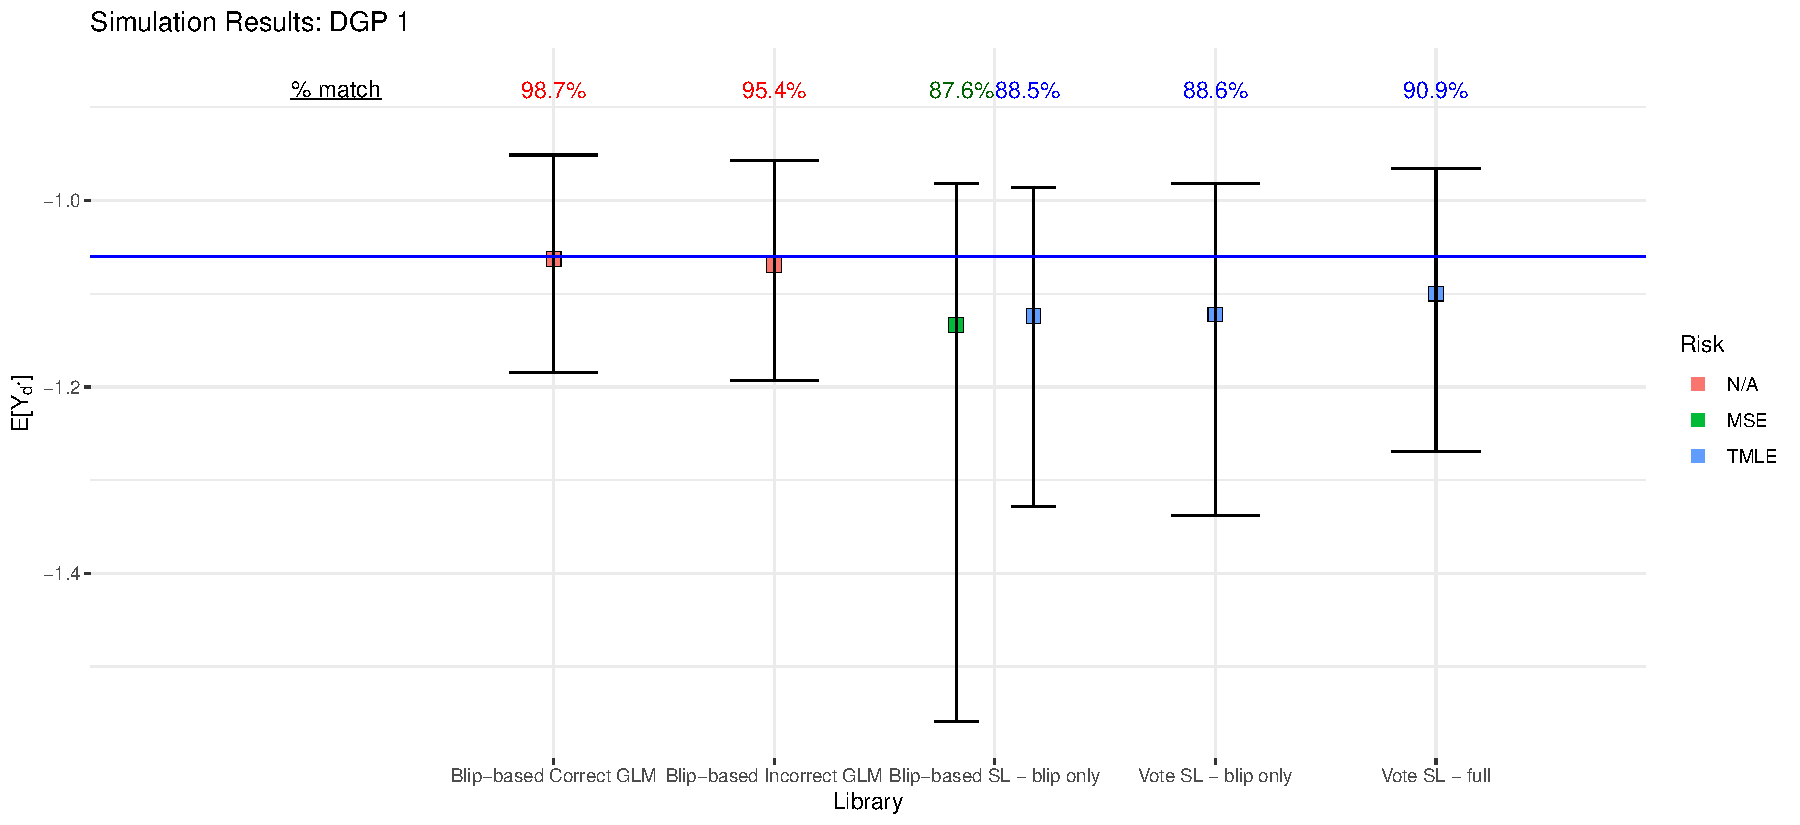
\includegraphics[width=\maxwidth]{figure/ODTR_DGP_smooth_step1a-1} 
% latex table generated in R 3.5.1 by xtable 1.8-4 package
% Sat Aug 31 08:47:58 2019
\begin{table}[ht]
\centering
\scalebox{0.8}{
\begin{tabular}{rrr}
  \hline
 & MSE & TMLE \\ 
  \hline
Bias & -0.06021 & -0.05566 \\ 
  Variance & 0.01432 & 0.00755 \\ 
  MSE & 0.01794 & 0.01064 \\ 
  coef.SL.glm & 0.51923 & 0.29013 \\ 
  coef.SL.mean & 0.10736 & 0.10224 \\ 
  coef.SL.glm.interaction & 0.09462 & 0.15061 \\ 
  coef.SL.earth & 0.07752 & 0.10576 \\ 
  coef.SL.nnet & 0.07717 & 0.12947 \\ 
  coef.SL.svm & 0.04754 & 0.08328 \\ 
  coef.SL.rpart & 0.07657 & 0.13851 \\ 
   \hline
\end{tabular}
}
\caption{smooth - step1a} 
\end{table}


\subsection{vote-based SL (b)}

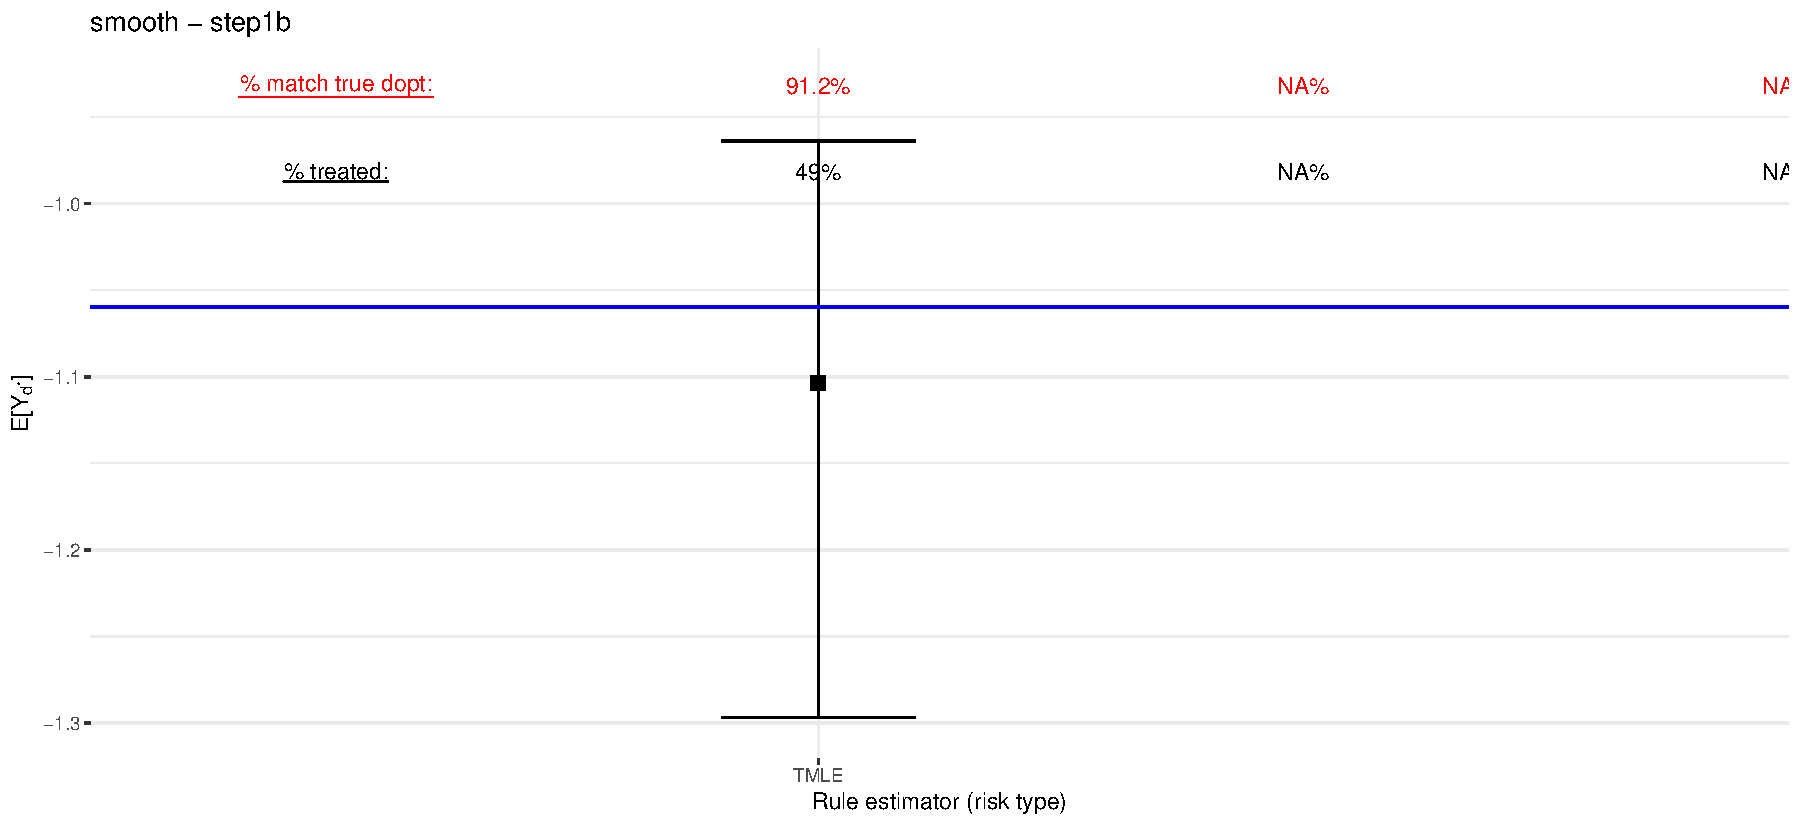
\includegraphics[width=\maxwidth]{figure/ODTR_DGP_smooth_step1b-1} 
% latex table generated in R 3.5.1 by xtable 1.8-4 package
% Sat Aug 31 08:47:58 2019
\begin{table}[ht]
\centering
\scalebox{0.7}{
\begin{tabular}{rr}
  \hline
 & TMLE \\ 
  \hline
Bias & -0.04396 \\ 
  Variance & 0.00865 \\ 
  MSE & 0.01057 \\ 
  coef.DonV.DonV.SL.glm\_All & 0.05479 \\ 
  coef.DonV.DonV.SL.mean\_All & 0.03260 \\ 
  coef.DonV.DonV.SL.glm.interaction\_All & 0.05291 \\ 
  coef.DonV.DonV.SL.earth\_All & 0.05614 \\ 
  coef.DonV.DonV.SL.nnet\_All & 0.05143 \\ 
  coef.DonV.DonV.SL.svm\_All & 0.04188 \\ 
  coef.DonV.DonV.SL.rpart\_All & 0.06386 \\ 
  coef.Qlearn.Qlearn.SL.glm\_All & 0.03504 \\ 
  coef.Qlearn.Qlearn.SL.mean\_All & 0.03906 \\ 
  coef.Qlearn.Qlearn.SL.glm.interaction\_All & 0.06912 \\ 
  coef.Qlearn.Qlearn.SL.earth\_All & 0.03911 \\ 
  coef.Qlearn.Qlearn.SL.nnet\_All & 0.04556 \\ 
  coef.Qlearn.Qlearn.SL.svm\_All & 0.03775 \\ 
  coef.Qlearn.Qlearn.SL.rpart\_All & 0.04111 \\ 
  coef.OWL & 0.04200 \\ 
  coef.EARL & 0.08225 \\ 
  coef.optclass & 0.06621 \\ 
  coef.RWL & 0.06807 \\ 
  coef.treatall & 0.04494 \\ 
  coef.treatnone & 0.03619 \\ 
   \hline
\end{tabular}
}
\caption{smooth - step1b} 
\end{table}








\section{Step 5}

\begin{itemize}
\item blip (a) and majority vote (b) SuperLearner
\item incorrect glm QAV, incorrect glm QAW
\end{itemize}



\subsection{Blip-based SL (a)}

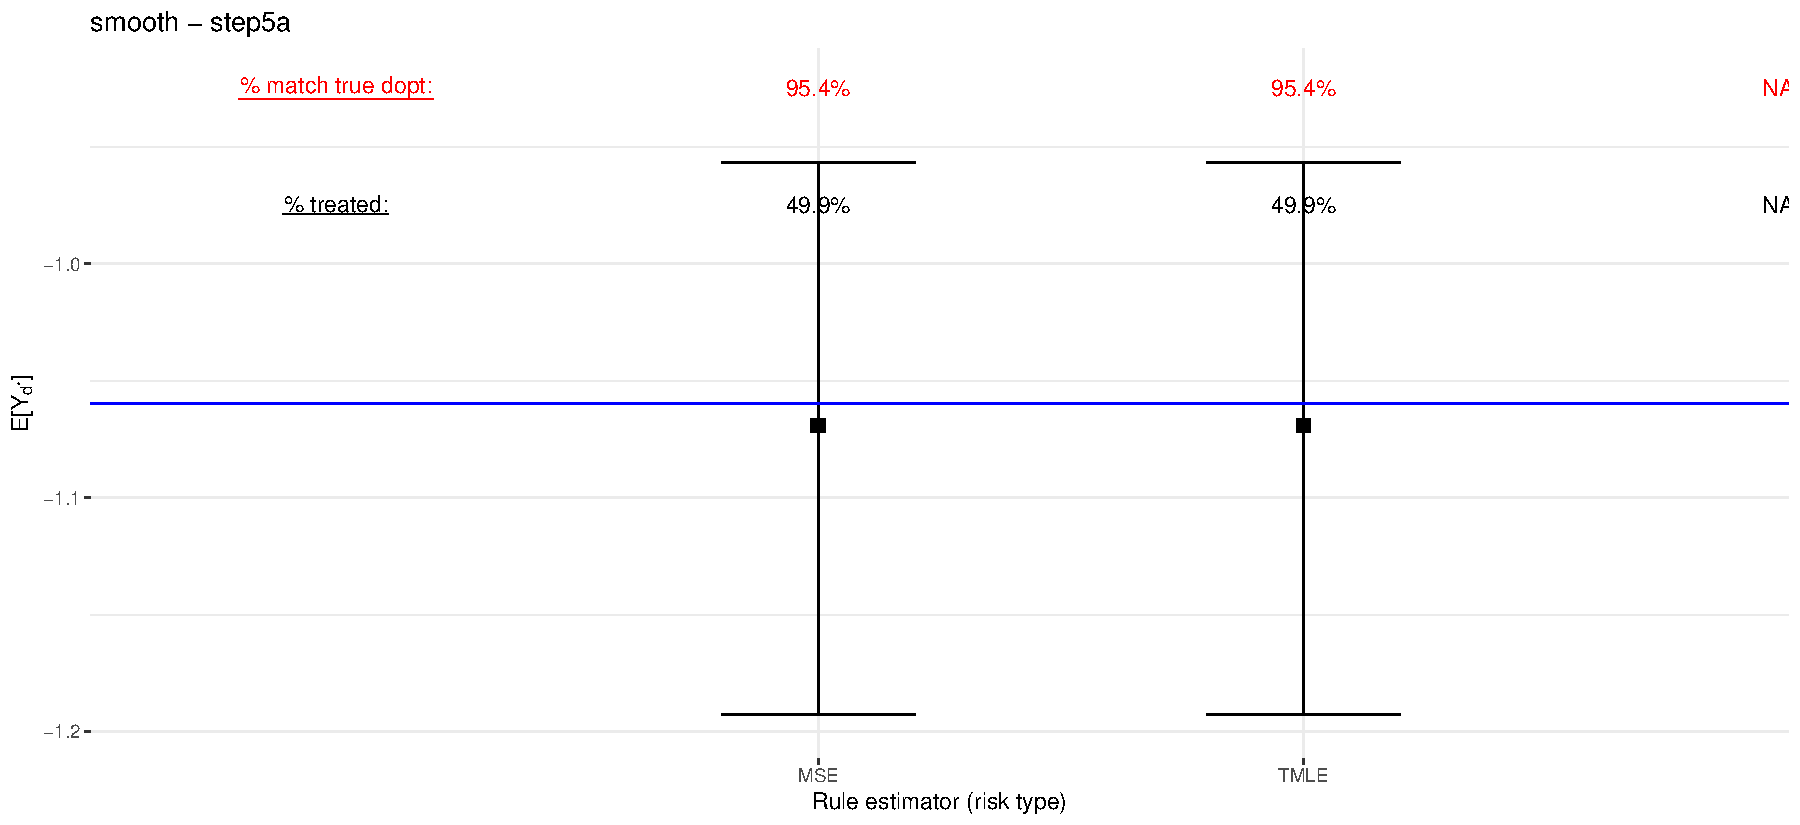
\includegraphics[width=\maxwidth]{figure/ODTR_DGP_smooth_step5a-1} 
% latex table generated in R 3.5.1 by xtable 1.8-4 package
% Sat Aug 31 08:47:59 2019
\begin{table}[ht]
\centering
\scalebox{0.7}{
\begin{tabular}{rrr}
  \hline
 & MSE & TMLE \\ 
  \hline
Bias & -0.00944 & -0.00944 \\ 
  Variance & 0.00344 & 0.00344 \\ 
  MSE & 0.00352 & 0.00352 \\ 
  estimates..1.....grep.colnames.estimates..1.....pattern....coef... & 1.00000 & 1.00000 \\ 
   \hline
\end{tabular}
}
\caption{smooth - step5a} 
\end{table}


\subsection{vote-based SL (b)}

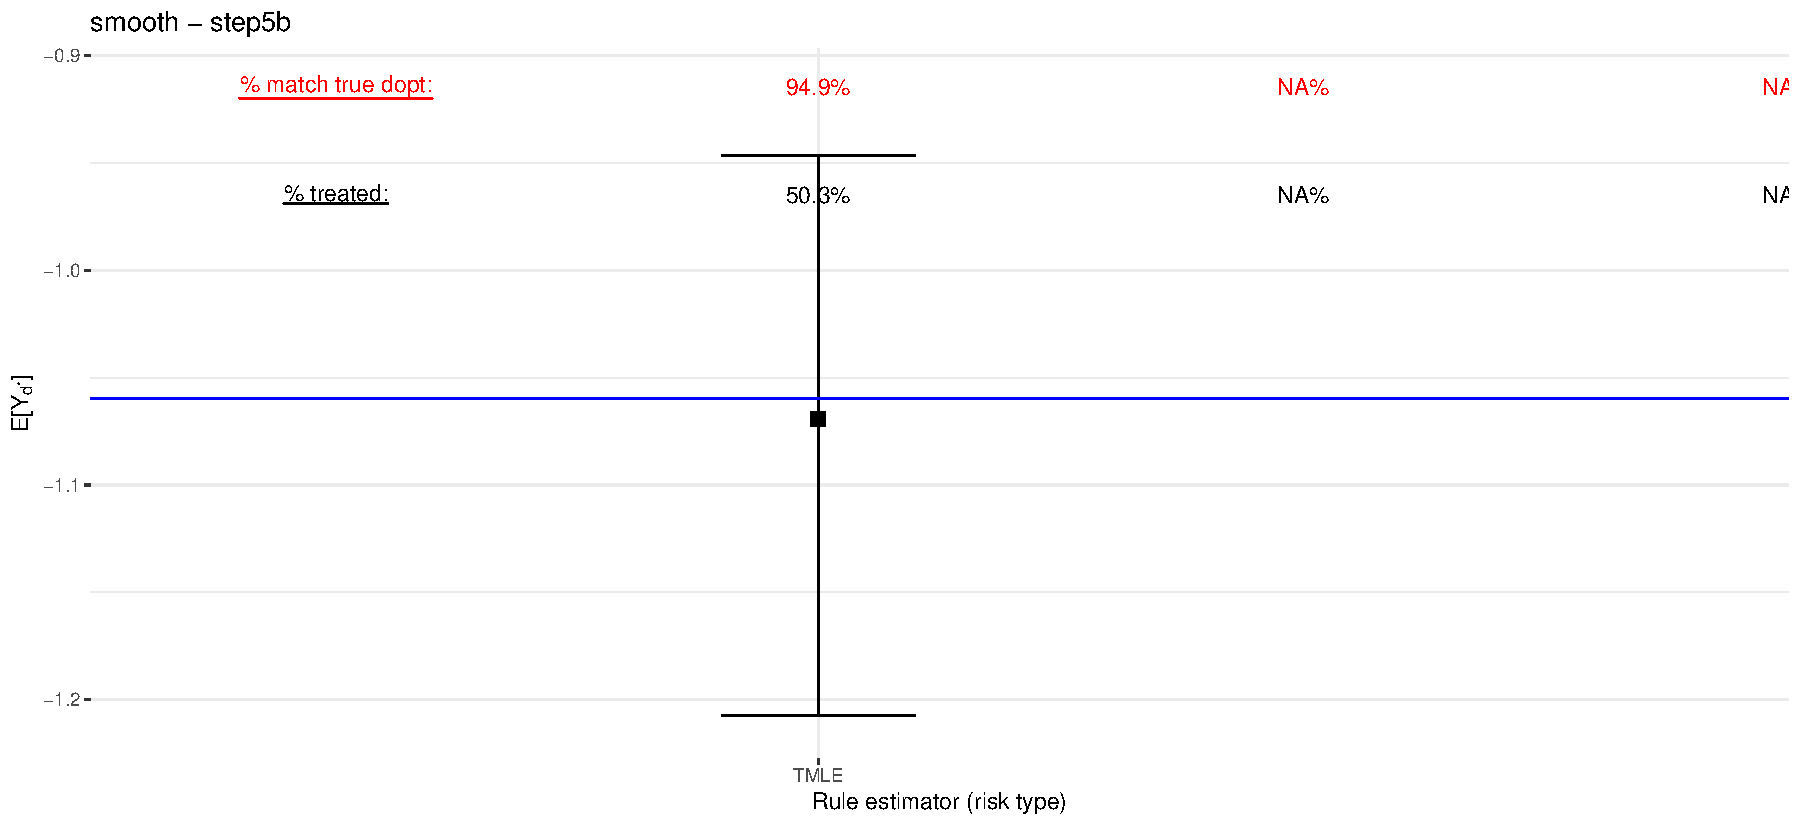
\includegraphics[width=\maxwidth]{figure/ODTR_DGP_smooth_step5b-1} 
% latex table generated in R 3.5.1 by xtable 1.8-4 package
% Sat Aug 31 08:47:59 2019
\begin{table}[ht]
\centering
\scalebox{0.7}{
\begin{tabular}{rr}
  \hline
 & TMLE \\ 
  \hline
Bias & -0.00978 \\ 
  Variance & 0.00466 \\ 
  MSE & 0.00475 \\ 
  coef.DonV.SL.glm\_All & 0.12644 \\ 
  coef.Qlearn.SL.QAW.incorrect\_All & 0.07654 \\ 
  coef.OWL & 0.07619 \\ 
  coef.EARL & 0.21256 \\ 
  coef.optclass & 0.13665 \\ 
  coef.RWL & 0.16684 \\ 
  coef.treatall & 0.07979 \\ 
  coef.treatnone & 0.12499 \\ 
   \hline
\end{tabular}
}
\caption{smooth - step5a} 
\end{table}


\end{document}
